\section{Modelo Computacional} \label{metodologia:modelocomputacional}

Usando todas las curvas de luz disponible para el sistema \atoObjId --- tanto de
Gaia como los datos recabados de Iturbide --- se puede generar un modelo
computacional cuyas propiedades físicas pueden adecuadamente explicar los datos
observacionales. Este método al final daría como resultado una \textit{solución
fotométrica} del sistema. En el mejor de los casos, esta solución muestra un
valor satisfactorio de ajuste a los datos observacionales. A continuación se
plasma el proceso que se llevó a cabo para llegar a una solución fotométrica del
sistema \atoObjIdNoSpace; esta solución no es única en el sentido que otra
combinación de parámetros podría llegar a las mismas conclusiones.

\subsection{Estimaciones Iniciales}
\label{metodologia:modelocomputacional:estimacionesiniciales}

Una vez determinado el periodo orbital del sistema se puede empezar un estudio
de la morfología de las curvas de luz en fase. PHOEBE para facilitar esto ofrece
distintos métodos para generar los las primeras estimaciones de parámetros
físicos del sistema. El estimador \textbf{EBAI-KNN} para estimar los siguientes
parámetros: el \textit{tiempo de conjunción superior} (\code{t0\_supconj}), la
\textit{razón de temperaturas} (\code{teffratio}), la \textit{inclinación
orbital} (\code{incl@binary}), el \textit{factor de relleno}
(\quotes{\textit{fillout factor}} en inglés, \code{fillout\_factor}), y la
\textit{razón de masas} (\code{q}). A pesar que dentro de PHOEBE estén
implementados estimadores adicionales, solo se puede aplicar el
\textbf{EBAI-KNN} estimador; esto se debe a que el modelo del sistema del que
parte este trabajo corresponde al de una binaria en contacto (elegido por la
morfología aparente de la curva de luz de Iturbide).

Dentro del Jupyter Notebook
\href{https://github.com/KnightIV/UANL_MAPTA_PlanObservaciones/blob/main/analisis/phoebe_model/estimations/ebai-default.ipynb}{\code{ebai-default.ipynb}}
se puede encontrar el código con el que se llevaron a cabo las pruebas de
estimación de parámetros. El estimador \textbf{EBAI-KNN} puede que obtenga
diferentes soluciones del sistema dependiendo de la curva de luz utilizada; por
lo cual se esperaba que obtuviera diferentes resultados dependiendo de la curva
de entrada. Para obtener un panorama completo de las posibles soluciones
fotométricas so ejecutaron varios estimadores de PHOEBE, cada uno operando sobre
una diferente combinación de curvas de luz; se corrió un estimador por cada
curva de luz individual, al igual que unos estimadores que tuvieron de entrada
una combinación de curvas de luz de Gaia e Iturbide. El experimento completo
junto a sus curvas de luz sintéticas correspondientes se pueden ver en el
Notebook antedicho, acompañado de las gráficas resultantes de cada estimador.

\subsubsection{Elección de Modelo Inicial}
\label{metodologia:modelocomputacional:estimacionesiniciales:eligiendomodeloinicial}

Una consideración importante en el proceso de modelación computacional es la
existencia de diferentes soluciones fotométricas dado un mismo conjunto de
datos. Esto se debe a la ortogonalidad de los parámetros en el sistema; dos o
más parámetros pueden estar en un estado de degeneración, donde existe una
relación lineal entre estos, lo cual significa que no existe una solución única
correcta del sistema. Para decidir entre los varios estimadores se tomó como
criterio de selección el ajuste del "forward model" a los datos mediante la
estadística $\chi^2$. Estos se pueden ver en la figura \ref{chiSqrdFigure}.
Partiendo de la medición del ajuste de cada modelo se ve que
\code{ebai\_knn\_raw} y \code{ebai\_knn\_lc\_iturbide\_raw} son los que mejor se
acoplan a los datos observacionales. La optimización de parámetros se llevó a
cabo partiendo de las estimaciones de \code{ebai\_knn\_raw}, el cual de entrada
recibió las cuatro curvas de luz de este trabajo (3 de Gaia, 1 de Iturbide). El
resultado inicial del modelo se puede ver en la figura
\ref{ebaiKnnRawEstimateModel}, junto a los parámetros del modelo en la tabla \ref{ebaiKnnInitialEstimationsValues}.

\begin{figure}[!ht]
	\centering
	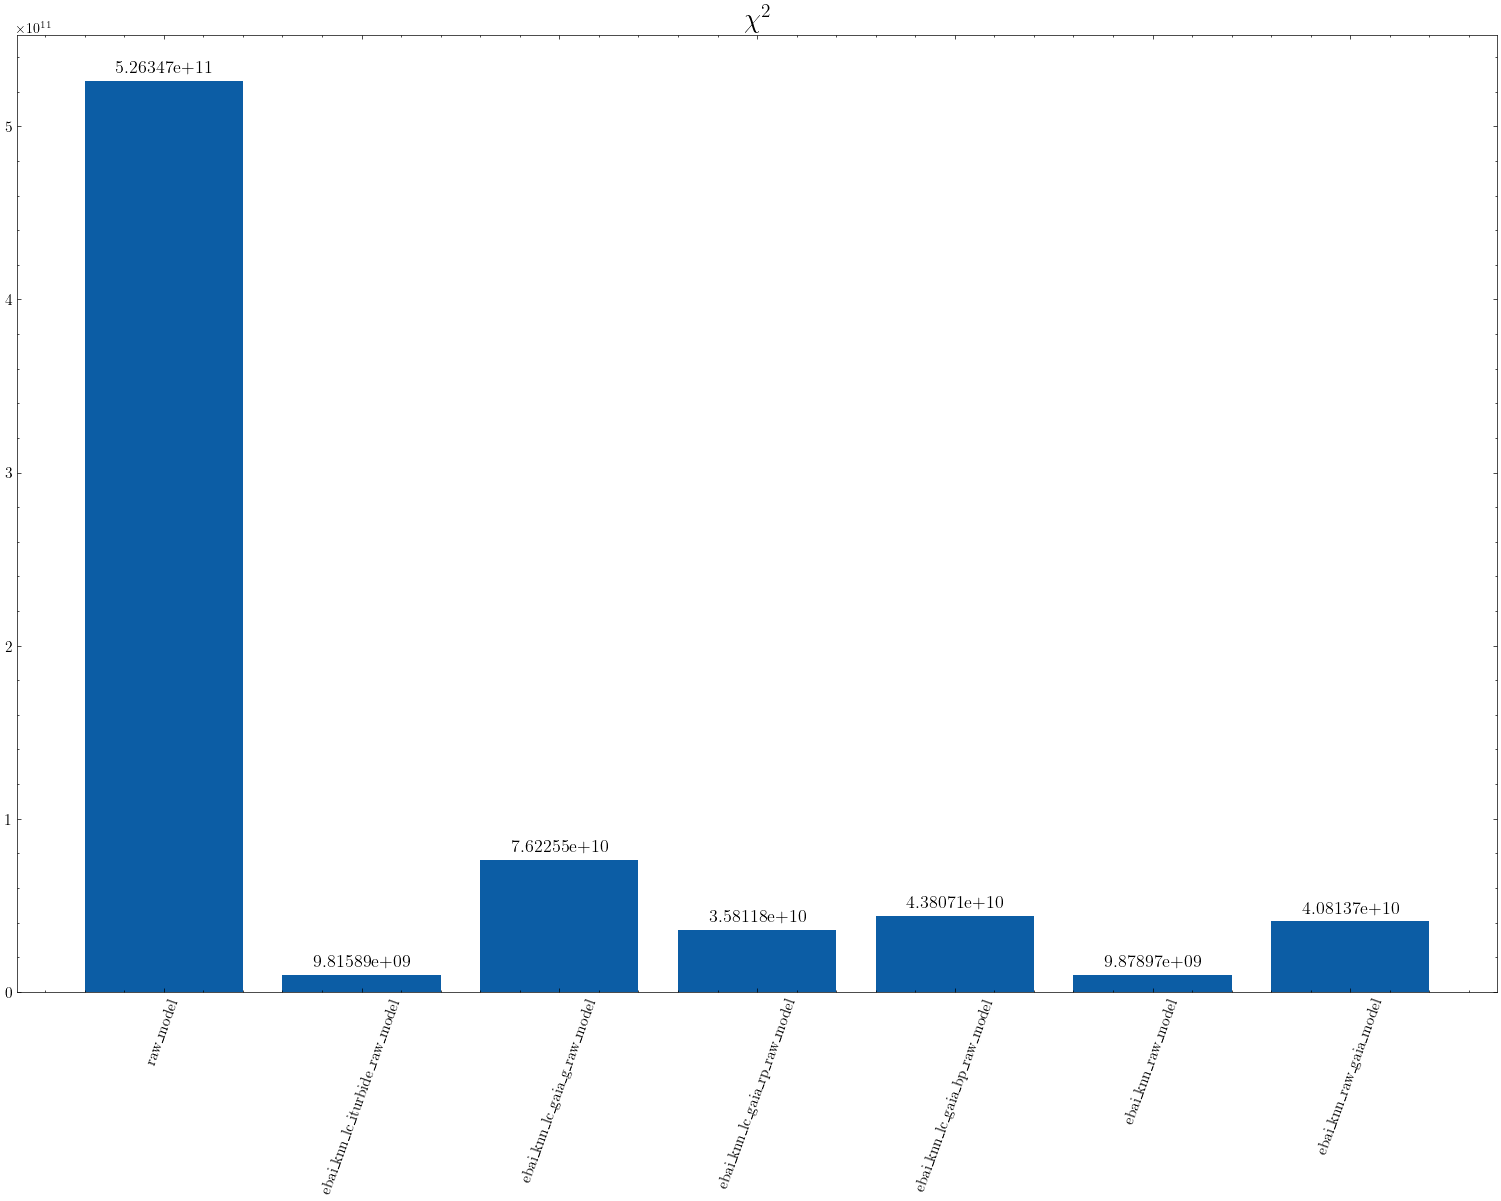
\includegraphics[scale=0.43]{Metodologia/Secciones/ModeloComputacional/Figures/EstimadoresChiResultados.png}
	
	\caption{Resultados de $\chi^2$ de los modelos sintéticos generados
	utilizando los parámetros de los estimadores. Cada estadística fue calculada
	con respecto a todos los datos observacionales disponibles, sin importar las
	combinaciones de curvas de luz utilizadas para hacer la estimación.
	\code{raw\_model} corresponde al modelo inicial que ofrece PHOEBE a través de
	la función \code{phoebe.default\_contact\_binary()}.} 
	\label{chiSqrdFigure}
\end{figure}

\begin{figure}[!ht]
	\centering
	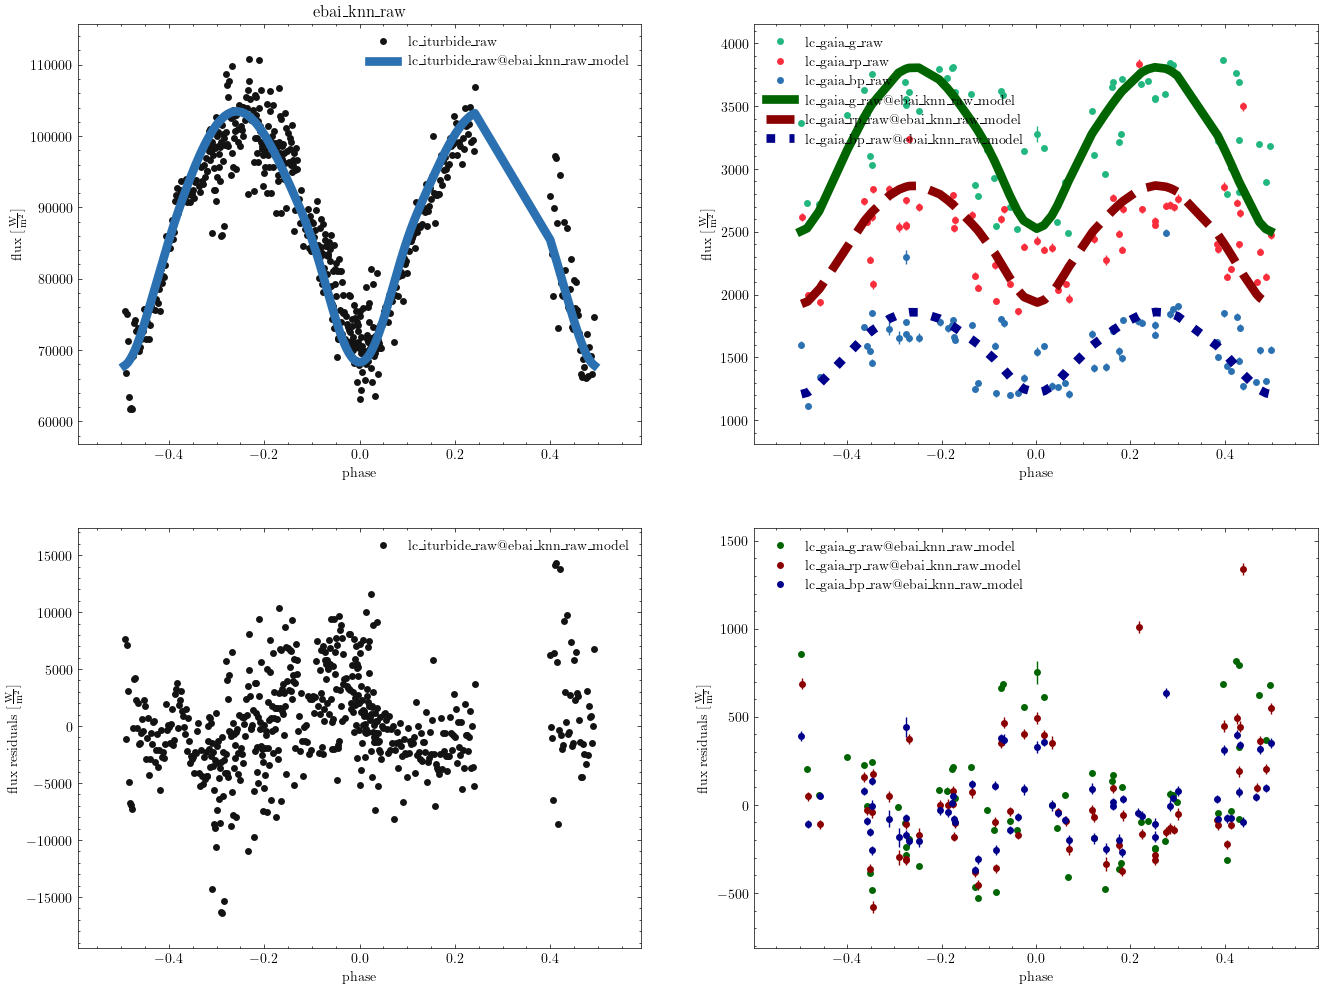
\includegraphics[scale=0.5]{Metodologia/Secciones/ModeloComputacional/Figures/ebai_knn_raw_estimacion.png}
	
	\caption{Modelos sintéticos del modelo utilizando los parámetros estimados
	por \code{ebai\_knn\_raw\_solver} junto a los residuos en los flujos para
	cada curva de luz. Estos modelos fueron sintetizados utilizando un factor de
	escala de flujos flexible, utilizando la opción \code{pblum\_mode =
	"dataset\_scaled"}, el cual nos permite analizar la morfología del modelo
	sintético sin considerar por ahora el efecto en la escala de la curva de
	parámetros relacionados con la luminosidad de cada componente, como las
	temperaturas absolutas de ambas estrellas. Estos parámetros son ajustados en
	los siguientes pasos de afinación del modelo.}
	\label{ebaiKnnRawEstimateModel}
\end{figure}

% TODO: style table
\begin{table}[!ht]
	\centering
	\begin{tabular}{|l|l|}
		\hline
		% \rowcolor{blue}
		\thead{Parámetro} & \thead{Valor} \\
		\hline
		\code{t0\_supconj@binary} & 0.06841 d \\
		\hline
		\code{teffratio@binary} & 0.99560 \\
		\hline
		\code{incl@binary} & 1.25572 rad \\
		\hline
		\code{fillout\_factor@contact\_envelope} & 0.51640 \\
		\hline
		\code{q@binary} & 3.49495 \\
		\hline

	\end{tabular}
	\caption{Resultados adoptados de las estimaciones iniciales, utilizando el estimador cuyos datos de entrada fueron las cuatro curvas de luz disponibles. Las unidades de cada valor son especificadas excepto para los parámetros adimensionales.}
	\label{ebaiKnnInitialEstimationsValues}
\end{table}

% \begin{table}
% 	\centering
% 	\begin{tabular}{|l|l|l|l|l|l|l|}
% 		\hline
% 		  & \code{t0\_supconj} & \code{teffratio} & \code{incl@binary} & \code{fillout\_factor} & \code{q} \\ \hline
% 		\thead{Iturbide}               & 1 & 2 \\ \hline
% 		\thead{Iturbide (Normalizada)} & 3 & 4 \\ \hline
% 		\thead{Gaia G}                       &  & 5 \\ \hline
% 		\thead{Gaia G (Normalizada)} \\ \hline
% 		\thead{Gaia G\textsubscript{RP}} &  6 & \\ \hline
% 		\thead{Gai G\textsubscript{RP} (Normalizada)} \\ \hline

% 	\end{tabular}
% 	\caption{EBAI KNN Estimaciones}
% \end{table}